\documentclass[12pt]{article}
\usepackage{mathtools,amssymb, amsthm, tikz}
\usetikzlibrary{angles, quotes, decorations.pathreplacing, arrows.meta}
\usepackage[margin=1in]{geometry}
\usepackage[T1]{fontenc}
\usepackage[utf8]{inputenc}
\usepackage[magyar]{babel}
\usepackage{icomma}
\usepackage{lmodern}
\usepackage{fontspec}
\setmainfont{Times New Roman}
\usepackage[linesnumbered,ruled,plain,longend]{algorithm2e}
\usepackage[hidelinks]{hyperref} 
\usepackage{wrapfig}
\usepackage{enumitem}
\usepackage{caption}
\usepackage{tabto}
\usepackage[style=numeric, backend=biber]{biblatex}
\addbibresource{forrasok.bib}
\usepackage{pgfplots}
\pgfplotsset{compat=1.18}

\captionsetup[figure]{
    labelfont=bf,
    name=Ábra,
    labelsep=newline,
    justification=centering,
    singlelinecheck=false
}

\newcommand{\assign}{\leftarrow}

% Algoritmus név
\SetAlgorithmName{Algoritmus}{Algoritmusok}{Algoritmus}
\SetAlgoCaptionSeparator{:} 
\makeatletter
\renewcommand{\fnum@algocf}{\AlCapSty{\AlCapFnt\thealgocf.\nobreakspace\algorithmcfname}}
\makeatother

% Függvények
\SetKwProg{Eljaras}{Eljárás}{:}{Eljárás vége}
\SetKwProg{Fuggveny}{Függvény}{}{Függvény vége}

% Változók
\SetKwInput{Valtozok}{Változó}
\SetKwInput{Konstansok}{Konstans}
\SetKwInput{Tipus}{Típus}
\SetKwInput{Be}{Be}
\SetKwInput{Ki}{Ki}

% Ciklusok
\SetKwFor{Ciklus}{Ciklus}{}{Ciklus vége}
\SetKwFor{CiklusAmig}{Ciklus amíg}{}{vége}

% Elágazás
\SetKwIF{Ha}{}{Kulonben}{Elágazás}{akkor}{Különben}{}{Elágazás vége}

% Logikai operátorok
\SetKw{Es}{$\wedge$}
\SetKw{Vagy}{$\vee$}
\SetKw{Nem}{$\neg$}

% Tömb
\SetKw{Tomb}{tömb}

% Komment
\SetKwComment{Komment}{[}{]}

\title{Perlin-zaj}
\author{Pintér Bálint}
\renewcommand{\contentsname}{Tartalomjegyzék}

\begin{document}
\maketitle
\newpage
\tableofcontents
\newpage

\section{Perlin-zaj}
A Perlin-zaj \textsuperscript{\cite{10.1145/325165.325247}} egy gradiensalapú
zajgenerálási algoritmus, amelynek a célja véletlenszerű, mégis összefüggő zaj
létrehozása. Segítségével a természetben előforduló véletlenszerű jelenségeket
lehet jól szimulálni, mint például domborzatokat, felhőket vagy a víz
hullámzását. Tetszőleges $n$ dimenzióra létrehozható, de jellemzően az elsőtől
a negyedik dimenzióig alkalmazzák. A kódban egy kétdimenziós Perlin-zaj van
implementálva.
\subsection{Működése összefoglalva}
\begin{enumerate}[noitemsep]
    \item \textbf{Rács meghatározása:} A zaj dimenziójában egy egész koordináták által kijelölt elméleti rácsot használunk, amelynek minden sarkához egy véletlenszerűen kiválasztott egységvektort rendelünk.
    \item \textbf{Rácsnégyzeten belüli vektorok kiszámítása:} Meghatározzuk a sarkokból a belső pontba mutató vektorokat.
    \item \textbf{Skaláris szorzás:} Az adott sarokból a pontba mutató vektornak és az adott sarokhoz rendelt vektornak vesszük a skaláris szorzatát.
    \item \textbf{Interpoláció:} A kapott skaláris szorzatokat végül tengelyenként interpoláljuk. Az interpoláció súlyozásához egy simítófüggvényt használunk. Például a kétdimenziós zajnál először az $x$ tengely mentén interpolálunk, majd a kapott részeredményeket az $y$ tengely mentén interpoláljuk.
\end{enumerate}
\section{Előkészítés}
A Perlin-zaj hatékony generálásához két adat inicializálására van szükség: egy
gradienstáblára és egy permutációs táblára. \newpage
\subsection{Gradienstábla}
A Perlin-zaj egy úgynevezett gradiensalapú zaj. Eszerint rácspontokat
határozunk meg, amelyekhez véletlenszerű vektorokat rendelünk. A gradienstábla
256 darab ilyen vektort tárol el. A vektorok dimenziószáma megegyezik a zaj
dimenziószámával. (Például: Kétdimenziós zaj esetén kétdimenziós vektorokat
használunk.)\\ \vspace{-8pt}
\begin{minipage}[t]{0.6\textwidth}
    \vspace{0pt}
    \begin{algorithm}[H]
        \linespread{0.65}\selectfont
        \caption{Gradienstábla létrehozása}
        \DontPrintSemicolon
        \LinesNotNumbered
        \Konstansok{MaxG = $256$}
        \Tipus{VéletlenSzámGenerátor = Osztály (\\
        \setlength\parindent{24pt} jelenlegiSzám: Egész\\
        \setlength\parindent{24pt} \textbf{Függvény} Következő: Egész\\
        \setlength\parindent{24pt} \textbf{Függvény} KövetkezőValós: Valós \Komment*[r]{$\in[0;1[$} \\
        )}
        \LinesNumbered
        \Tipus{Vektor = Rekord (\\
            \setlength\parindent{24pt} x: Valós\\
            \setlength\parindent{24pt} y: Valós\\
            )}
        \Eljaras{GradiensTablaGeneral (\textbf{Változó}: GradiensTabla: Tömb($1$..MaxG: Vektor),
            Rand: VéletlenSzámGenerátor)}{
            % Változók
            \Valtozok{$i$: Egész}
            \Ciklus{$i \coloneqq 1$-től $256$-ig}{
                GradiensTabla[$i$] $\coloneqq$ VeletlenVektorGeneral(Rand)
            }
        }
    \end{algorithm}
\end{minipage}
\hfill
\begin{minipage}[t]{0.4\textwidth}
    \vspace{0pt}
    \centering
    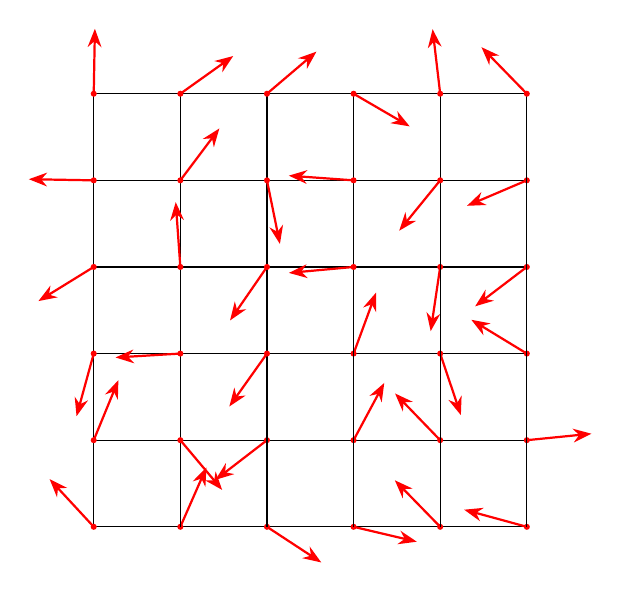
\begin{tikzpicture}[scale=0.55]
        \pgfmathsetseed{3432}
        \foreach \i in {0, 2, ..., 10} {
        \draw (\i, 0) -- (\i, 10);
        \draw (0, \i) -- (10, \i);
        \foreach \x in {0, 2, ..., 10} {
        \draw[-{Stealth}, red, thick] (\x,\i) -- ++(rnd*360:1.5);
        \fill[red] (\x,\i) circle (2pt);
        }
        }

    \end{tikzpicture}
    \captionof{figure}{A zaj rácsának szemléltetése.}
\end{minipage}
\vspace{-14pt}
\subsubsection{Vektorgenerálás}
Generálunk egy véletlenszerű számot $[0;2\pi[$ intervallumban. Majd egyszerű
trigonometriával a szöget egy vektorrá alakítjuk, ahol a vektor $x$ komponense
a véletlen szög koszinusza, és az $y$ komponense a szög szinusza. \\
\vspace{-8pt}
\begin{minipage}[t]{0.7\textwidth}
    \vspace{0pt}
    \begin{algorithm}[H]
        \linespread{0.55}\selectfont
        \caption{Véletlenszerű vektor generálás}
        \DontPrintSemicolon
        \Tipus{VéletlenSzámGenerátor = Osztály (\\
        \setlength\parindent{24pt} jelenlegiSzám: Egész\\
        \setlength\parindent{24pt} \textbf{Függvény} Következő: Egész\\
        \setlength\parindent{24pt} \textbf{Függvény} KövetkezőValós: Valós \Komment*[r]{$\in[0;1[$} \\
        )}
        \Tipus{Vektor = Rekord (\\
            \setlength\parindent{24pt} x: Valós\\
            \setlength\parindent{24pt} y: Valós\\
            )}

        \Fuggveny{VeletlenVektorGeneral (\textbf{Változó}: Rand: VéletlenSzámGenerátor): Vektor}{
            \Valtozok{szog: Valós}
            \Valtozok{vektor: Vektor}
            szog $\coloneqq$ Rand.KövetkezőValós() $* 2 * \pi$\\
            vektor.x $\coloneqq \cos(\text{szog})$\\
            vektor.y $\coloneqq \sin(\text{szog})$\\
            \textit{VeletlenVektorGeneral} $\coloneqq$ vektor
        }
    \end{algorithm}
\end{minipage}
\hfill
\begin{minipage}[t]{0.3\textwidth}
    \vspace{0pt}
    \centering
    \hspace*{0.6cm}
    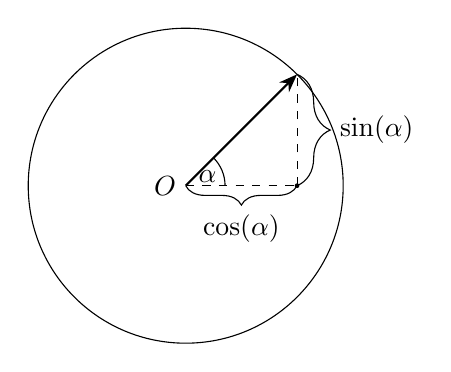
\begin{tikzpicture}[scale=2]
        \coordinate (O) at (0,0);
        \draw (O) circle (1cm);
        \pgfmathsetmacro{\angle}{45}
        \pgfmathsetmacro{\x}{cos(\angle)}
        \pgfmathsetmacro{\y}{sin(\angle)}
        \fill[black] (\x,0) circle (0.15mm);
        \draw[-{Stealth}, black, thick] (O) -- (\x, \y);
        \coordinate (A) at (\x, \y);
        \coordinate (B) at (\x, 0);
        \draw pic ["$\alpha$", draw=black, angle radius=5mm] {angle = B--O--A};
        \draw[dashed] (O) -- (B);
        \draw[decorate, decoration={brace, mirror, amplitude=7pt}]
        (O) -- (B) node[midway, below=7pt] {$\cos(\alpha)$};
        \draw[dashed] (B) -- (A);
        \draw[decorate, decoration={brace, mirror, amplitude=12pt}]
        (B) -- (A) node[midway, right=12pt] {$\sin(\alpha)$};

        \node[left] at (O) {$O$};
    \end{tikzpicture}
    \captionof{figure}{A vektorok előállításának szemléltetése.}
\end{minipage}
\newpage
\subsection{Permutációs tábla}
A permutációs tábla kezdetben $0$-tól $255$-ig tartalmazza a számokat növekvő
sorrendben. Ezt a listát egy véletlenszám-generátor segítségével összekeverjük
és önmaga után fűzzük (ezzel egy $512$ elemű tömböt kapunk). Így a hashelésnél
elkerülhető a túlindexelés, amely gyorsítja a zajgenerálást, mivel elhagyható a
határellenőrzés. \\
\begin{algorithm}[H]
    \caption{Permutációs tábla létrehozása}
    \DontPrintSemicolon
    \Konstansok{MaxP = $512$}
    \Tipus{VéletlenSzámGenerátor = Osztály (\\
    \setlength\parindent{24pt} jelenlegiSzám: Egész\\
    \setlength\parindent{24pt} \textbf{Függvény} Következő: Egész\\
    \setlength\parindent{24pt} \textbf{Függvény} KövetkezőValós: Valós \Komment*[l]{$\in[0;1[$} \\
    )}

    \Eljaras{PermutaciosTablaGeneral (\textbf{Változó}: PermutaciosTabla: Tömb($1$..MaxP: Egész),
        Rand: VéletlenSzámGenerátor)}{
        % Változók
        \Valtozok{$i$, $j$, temp: Egész}
        \Ciklus{$i \coloneqq 1$-től $256$-ig}{
            PermutaciosTabla[$i$] $\coloneqq i - 1$
        }
        \;
        \Ciklus{$i \coloneqq 256$-tól $2$-ig $-1$-esével}{
            j $\coloneqq$ (Rand.Következő() Mod $i$) + 1  \\
            temp $\coloneqq$ PermutaciosTabla[$i$] \\
            PermutaciosTabla[$i$] $\coloneqq$ PermutaciosTabla[$j$] \\
            PermutaciosTabla[$j$] $\coloneqq$ temp \\
        }
        \;
        \Ciklus{$i \coloneqq 1$-től $256$-ig}{
            PermutaciosTabla[$i + 256$] $\coloneqq$ PermutaciosTabla[$i$]
        }
    }
\end{algorithm}
\newpage
\section{Zajszámítás}
\subsection{Rácspontok meghatározása}
\begin{wrapfigure}{r}{0.6\textwidth}
    \centering
    \vspace{-40pt}
    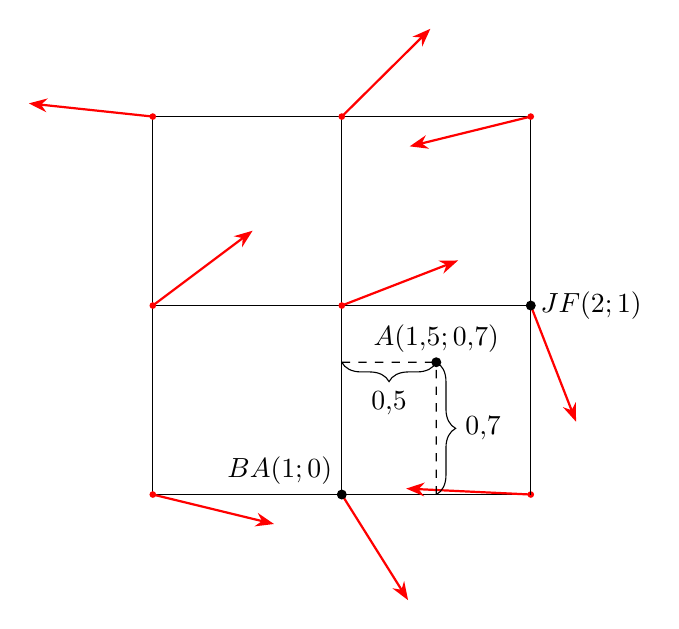
\begin{tikzpicture}[scale=0.6]
        \pgfmathsetseed{10}
        \pgfmathsetmacro{\racsok}{8}
        \pgfmathsetmacro{\racsokSzama}{2}
        \pgfmathsetmacro{\meret}{4}
        \foreach \i in {0, \meret, ..., \racsok} {
        \draw (\i, 0) -- (\i, \racsok);
        \draw (0, \i) -- (\racsok, \i);
        \foreach \x in {0, \meret, ..., \racsok} {
        \draw[-{Stealth}, red, thick] (\x,\i) -- ++(rnd*360:{\meret*0.66});
        \fill[red] (\x,\i) circle (2pt);
        }
        }

        \coordinate (A) at ({\meret + \meret * 0.5}, {\meret * 0.7});
        \fill (A) circle (3pt);
        \node[above] at (A) {$A(1,5;0,7)$};
        \coordinate (B) at (\meret, 0.0);
        \fill (B) circle (3pt);
        \node[above left] at (B) {$BA(1;0)$};
        \coordinate (C) at ({\meret * 2}, \meret);
        \fill (C) circle (3pt);
        \node[right] at (C) {$JF(2;1)$};

        \draw[dashed] (\meret, {\meret * 0.7}) -- (A);
        \draw[decorate, decoration={brace, mirror, amplitude=7pt}]
        (\meret, {\meret * 0.7}) -- (A) node[midway, below=7pt] {$0,5$};
        \draw[dashed] ({\meret + \meret * 0.5}, 0.0) -- (A);
        \draw[decorate, decoration={brace, mirror, amplitude=7pt}]
        ({\meret + \meret * 0.5}, 0.0) -- (A) node[midway, right=7pt] {$0,7$};
    \end{tikzpicture}
    \\
    \caption{A rácspont koordinátáinak szemléltetése.}
    \vspace{10pt}
\end{wrapfigure}
Először meghatározzuk, hogy az adott ($x$, $y$) pont melyik négyzetbe esik. Ehhez a koordinátákat lefelé kerekítjük, majd az
eredményen elvégzünk egy $255$-tel való bitenkénti ÉS (AND) műveletet. Ez a művelet az eredményt a $[0;255]$
tartományba hozza: ha az érték nagyobb, mint $255$, akkor visszafordul az
intervallum elejére (pl. $256$-ból $0$ lesz, $257$-ből $1$ lesz). Ezt elvégezve az $x$-re és $y$-ra
megkapjuk a bal alsó rácspont koordinátáit.\\
A jobb felső rácspont koordinátáit úgy kapjuk meg, hogy a bal alsó pont értékeit $1$-gyel megnöveljük, majd az eredményt $255$-tel bitenkénti ÉS művelettel maszkoljuk.
A bitenkénti ÉS műveletre a túlcsordulás kezelése miatt van szükség.\\ A négyzeten belüli pontot úgy
kapjuk meg, hogy a számból kivonjuk annak lefelé kerekített értékét. \\ \\
Pszeudókódban megvalósítva:
\begin{algorithm}
    \caption{Rácspontok és négyzeten belüli koordináták kiszámítása}
    \DontPrintSemicolon

    \Tipus{Rácspont = Rekord (\\
        \setlength\parindent{24pt} balAlsóPontX, balAlsóPontY: Egész\\
        \setlength\parindent{24pt} jobbFelsőPontX, jobbFelsőPontY: Egész\\
        \setlength\parindent{24pt} relatívX, relatívY: Valós\\
        )}
    \Fuggveny{RacspontKiszamolasa(\textbf{Konstans}: $x$, $y$: Valós) : Rácspont}{
        \Valtozok{jelenlegiRácspont: Rácspont}
        jelenlegiRácspont.balAlsóPontX $\coloneqq$ floor($x$) \& $255$ \\
        jelenlegiRácspont.balAlsóPontY $\coloneqq$ floor($y$) \& $255$ \\
        jelenlegiRácspont.jobbFelsőPontX $\coloneqq$ (jelenlegiRácspont.balAlsóPontX $+ 1$) \& $255$ \\ jelenlegiRácspont.jobbFelsőPontY $\coloneqq$
        (jelenlegiRácspont.balAlsóPontY $+ 1$) \& $255$ \\
        \;
        jelenlegiRácspont.relatívX $\coloneqq x -$ floor($x$) \\
        jelenlegiRácspont.relatívY $\coloneqq y -$ floor($y$)
        \;
        \textit{RacspontKiszamolasa} $\coloneqq$ jelenlegiRácspont
    }
\end{algorithm}
\subsection{Skaláris szorzat kiszámítása}
\subsubsection{Gradiens vektorok kiválasztása}
A gradiens vektorokat a permutációs tábla és a \textit{Hash} függvény
segítségével választjuk ki. Vesszük a permutációs tábla $x$-edik elemét,
hozzáadjuk az $y$ értékét, majd ezt az összeget használjuk indexként a
permutációs táblában. Az így kapott eredmény lesz az indexe a gradiens
vektornak a gradienstáblából.
\begin{algorithm}
    \linespread{0.75}\selectfont
    \caption{Gradiens vektor kiválasztása}
    \DontPrintSemicolon
    \Tipus{Vektor = Rekord (\\
        \setlength\parindent{24pt} x: Valós\\
        \setlength\parindent{24pt} y: Valós\\
        )}
    \Konstansok{MaxP = $512$, MaxG = $256$}
    \Valtozok{PermutaciosTabla: Tömb($1$..MaxP: Egész)}
    \Valtozok{GradiensTabla: Tömb($1$..MaxG: Vektor)\\}

    \Fuggveny{Hash(\textbf{Konstans}: $x$, $y$: Egész) : Egész}{
        \Komment{A permutációs tábla 0-tól 255-ig tartalmazza a számokat}
        \Komment{Azonban a pszeudókód 1-től kezdi az indexelést, ezért hozzáadunk egyet}
        \textit{Hash} $\coloneqq$ PermutaciosTabla[(PermutaciosTabla[$x$] + 1) + $y$] + 1
    }
    \;
    \Fuggveny{GradiensVektorKivalaszt(\textbf{Konstans}: $x$, $y$: Egész) : Vektor}{
        \Komment{A rácspont koordináták $[0;255]$ intervallumba esnek}
        \Komment{Azonban a pszeudókód 1-től kezdi az indexelést, ezért hozzáadunk egyet}
        \textit{GradiensVektorKivalaszt} $\coloneqq$ GradiensTabla[Hash($x + 1$, $y + 1$)]
    }
\end{algorithm}
\subsubsection{A sarkokból a pontba mutató vektorok kiszámítása}
Legyen a négyzeten belüli $P$ pont relatív koordinátái $(x_{0}, y_{0})$, ahol
$x_{0}, y_{0} \in [0;1]$. A rácsnégyzet sarkai legyen $A, B, C, D$.\\ Így a
sarkokból a pontba mutató vektorok:

\noindent
\begin{minipage}[t]{0.5\textwidth}
    \vspace{0pt}
    \begin{itemize}[noitemsep, leftmargin=*]
        \item \textbf{Bal alsó:} \tabto{3cm} $\vec{v}_{AP}(x_{0}, y_{0})$
        \item \textbf{Jobb alsó:} \tabto{3cm} $\vec{v}_{BP}(x_{0}-1, y_{0})$
        \item \textbf{Bal felső:} \tabto{3cm} $\vec{v}_{DP}(x_{0}, y_{0}-1)$
        \item \textbf{Jobb felső:} \tabto{3cm} $\vec{v}_{CP}(x_{0}-1, y_{0}-1)$
    \end{itemize}
\end{minipage}
\begin{minipage}[t]{0.5\textwidth}
    \vspace{-15pt}
    \centering
    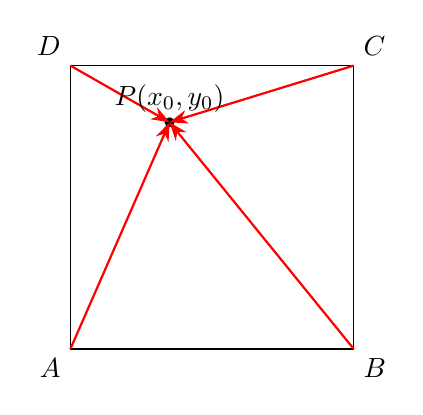
\begin{tikzpicture}[scale=0.9]
        \pgfmathsetseed{3432}
        \pgfmathsetmacro{\meret}{4}
        \coordinate (A) at (0, 0);
        \node[below left] at (A) {$A$};
        \coordinate (B) at (\meret, 0);
        \node[below right] at (B) {$B$};
        \coordinate (C) at (\meret, \meret);
        \node[above right] at (C) {$C$};
        \coordinate (D) at (0, \meret);
        \node[above left] at (D) {$D$};
        \draw (A) -- (B) -- (C) -- (D) -- cycle;

        \coordinate (P) at (1.4, 3.2);
        \fill (P) circle (2pt);
        \draw[-{Stealth}, red, thick] (A) -- (P);
        \draw[-{Stealth}, red, thick] (B) -- (P);
        \draw[-{Stealth}, red, thick] (C) -- (P);
        \draw[-{Stealth}, red, thick] (D) -- (P);
        \node[above] at (P) {$P (x_{0}, y_{0})$};

    \end{tikzpicture}
    \captionof{figure}{Relatív vektorok.}
\end{minipage}
\newpage
\subsubsection{Skaláris szorzat kiszámítása}
A vektorok meghatározása után kiszámítjuk az adott sarokhoz tartozó gradiens-
és relatív vektorok skaláris szorzatát. A skaláris szorzatot a matematikai
tétel alapján végezzük: $\vec{a} \cdot \vec{b} = x_{a}x_{b} + y_{a}y_{b} $
\begin{algorithm}[H]
    \caption{Skaláris szorzat}
    \DontPrintSemicolon
    \Tipus{Vektor = Rekord (\\
        \setlength\parindent{24pt} x: Valós\\
        \setlength\parindent{24pt} y: Valós\\
        )}
    \Fuggveny{SkalarisSzorzat(\textbf{Konstans}: $v1$, $v2$: Vektor) : Valós}{
        \textit{SkalarisSzorzat} $\coloneqq$ v1.x $*$ v2.x + v1.y $*$ v2.y
    }
\end{algorithm}
\subsection{Interpoláció}
A kapott skalárszorzatokat végül a simítófüggvény által módosított
súlytényezővel interpoláljuk a tengelyek mentén.
\subsubsection{Simítófüggvény}
Simítófüggvényként a Ken Perlin által 2002-ben, az `Improved Noise'-ban
\textsuperscript{\cite{10.1145/566654.566636}} bevezetett függvényt használjuk.
\[
    s(t) = 6t^{5} - 15t^{4} + 10t^{3}
\]
A függvény fontos jellemzője, hogy az első deriváltja és a második deriváltja
is egyenlő 0-val $t=0$ és $t=1$ esetén, így sima, folyamatos átmenet lesz a
rácsnégyzetek közt.\\
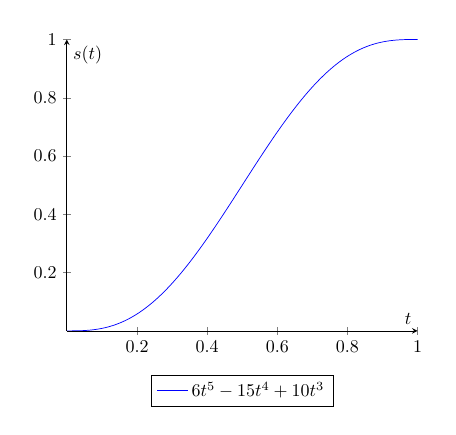
\begin{tikzpicture}[scale=0.65]
    \begin{axis}[
            axis lines = middle,
            xlabel = $t$,
            ylabel = {$s(t)$},
            legend style={
                    at={(0.5,-0.15)},
                    anchor=north,
                    legend columns=-1
                }
        ]
        \addplot [
            domain=0:1,
            samples=300,
            color=blue,
        ] {6*x^5 - 15*x^4 + 10*x^3};
        \addlegendentry{$6t^{5} - 15t^{4} + 10t^{3}$}
    \end{axis}
\end{tikzpicture}
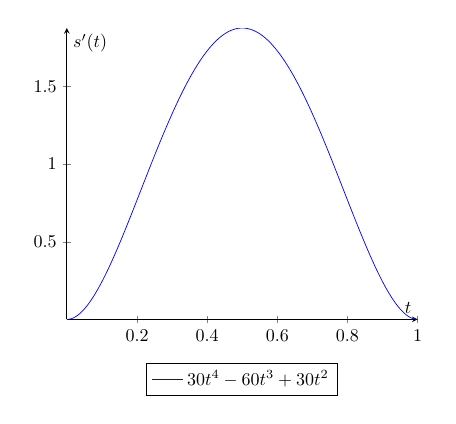
\begin{tikzpicture}[scale=0.65]
    \begin{axis}[
            axis lines = middle,
            xlabel = $t$,
            ylabel = {$s'(t)$},
            legend style={
                    at={(0.5,-0.15)},
                    anchor=north,
                    legend columns=-1
                }
        ]
        \addplot [
            domain=0:1,
            samples=300,
            color=blue,
        ] {30*x^4 - 60*x^3 + 30*x^2};
        \addlegendentry{$30t^{4} - 60t^{3} + 30t^{2}$}
    \end{axis}
\end{tikzpicture}
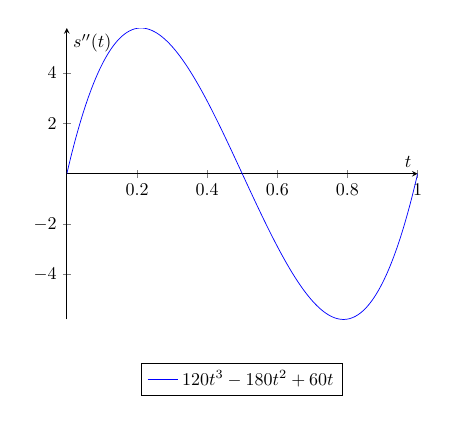
\begin{tikzpicture}[scale=0.65]
    \begin{axis}[
            axis lines = middle,
            xlabel = $t$,
            ylabel = {$s''(t)$},
            legend style={
                    at={(0.5,-0.15)},
                    anchor=north,
                    legend columns=-1
                }
        ]
        \addplot [
            domain=0:1,
            samples=300,
            color=blue,
        ] {120*x^3 - 180*x^2 + 60*x};
        \addlegendentry{$120t^{3} - 180t^{2} + 60t$}
    \end{axis}
\end{tikzpicture}
\begin{algorithm}
    \caption{Simítófüggvény}
    \DontPrintSemicolon
    \Fuggveny{Simitofuggveny(\textbf{Konstans}: t: Valós) : Valós}{
        \Komment{Horner-elrendezésben ($12$ szorzás helyett csak $5$ szorzás):}
        \textit{Simitofuggveny} $\coloneqq$ $t * t * t * (10 + t * ((-15) + t * 6))$
    }
\end{algorithm}
\subsubsection{Interpoláció}
A végeredményt a skaláris szorzatok interpolálásával kapjuk. Kétdimenziós
esetben először kiszámítjuk a relatív x-koordináta simítófüggvénybeli értékét,
majd eszerint interpoláljuk a skaláris szorzatokat az x tengely mentén, tehát a
felső két sarokhoz, illetve az alsó két sarokhoz tartozó skaláris szorzatokat
interpoláljuk egymással. Majd meghatározzuk a relatív y-koordináta
simítófüggvénybeli értékét, és eszerint interpoláljuk az előző két interpolált
részeredményt.
\begin{algorithm}
    \caption{Interpoláció}
    \DontPrintSemicolon
    \Fuggveny{Interpolacio(\textbf{Konstans}: a, b, t: Valós) : Valós}{
        \textit{Interpolacio} $\coloneqq$ $a + t * (b - a)$
    }
\end{algorithm}
\newpage
\section{Teljes zajfüggvény}
Először meghatározzuk a vizsgált pontot tartalmazó rácsnégyzet koordinátáit és
a ponton belüli relatív helyzetét a \textit{RacspontKiszamolasa} függvénnyel.
Ezt követően lekérjük a négy sarokhoz tartozó vektorokat a
\textit{GradiensVektorKivalaszt} függvénnyel, majd kiszámítjuk a sarkokból a
pontba mutató távolságvektorokat. Végül a \textit{SkalarisSzorzat} függvény
segítségével kiszámítjuk az egyes sarkokhoz tartozó relatív és gradiens
vektorok skaláris szorzatát. Legvégül interpoláljuk a skaláris szorzatokat az
\textit{Interpolacio} függvénnyel.
\begin{algorithm}
    \linespread{0.925}\selectfont
    \caption{Teljes zajfüggvény}
    \DontPrintSemicolon
    \Tipus{Vektor = Rekord (x, y: Valós)}
    \Tipus{Rácspont = Rekord (\\
        \setlength\parindent{24pt} balAlsóPontX, balAlsóPontY: Egész\\
        \setlength\parindent{24pt} jobbFelsőPontX, jobbFelsőPontY: Egész\\
        \setlength\parindent{24pt} relatívX, relatívY: Valós\\
        )}

    \Fuggveny{Zaj(\textbf{Konstans}: $x$, $y$: Valós) : Valós}{
        \Valtozok{rácspont: Rácspont}
        \Valtozok{g00, g10, g01, g11: Vektor}
        \Valtozok{v00, v10, v01, v11: Vektor}
        \Valtozok{tX, tY, a, b: Valós}
        \Komment{1. Rácspont és relatív koordináták kiszámítása}
        rácspont $\coloneqq$ RacspontKiszamolasa($x$, $y$)\\
        \Komment{2. Gradiens vektorok lekérdezése}
        g00 $\coloneqq$ GradiensVektorKivalaszt(rácspont.balAlsóPontX, rácspont.balAlsóPontY)\\
        g10 $\coloneqq$ GradiensVektorKivalaszt(rácspont.jobbFelsőPontX, rácspont.balAlsóPontY)\\
        g01 $\coloneqq$ GradiensVektorKivalaszt(rácspont.balAlsóPontX, rácspont.jobbFelsőPontY)\\
        g11 $\coloneqq$ GradiensVektorKivalaszt(rácspont.jobbFelsőPontX, rácspont.jobbFelsőPontY)\\
        \Komment{3. Relatív vektorok definiálása}
        v00.x $\coloneqq$ rácspont.relatívX\\
        v00.y $\coloneqq$ rácspont.relatívY\\
        v10.x $\coloneqq$ rácspont.relatívX - $1.0$\\
        v10.y $\coloneqq$ rácspont.relatívY\\
        v01.x $\coloneqq$ rácspont.relatívX\\
        v01.y $\coloneqq$ rácspont.relatívY - $1.0$\\
        v11.x $\coloneqq$ rácspont.relatívX - $1.0$\\
        v11.y $\coloneqq$ rácspont.relatívY - $1.0$\\
        \Komment{4. Simítófüggvény alkalmazása}
        tX $\coloneqq$ Simitofuggveny(rácspont.relatívX)\\
        tY $\coloneqq$ Simitofuggveny(rácspont.relatívY)\\
        \Komment{5. Skaláris szorzatok kiszámítása és interpolálásuk}
        a $\coloneqq$ Interpolacio(SkalarisSzorzat(g00, v00), SkalarisSzorzat(g10, v10), tX)\\
        b $\coloneqq$ Interpolacio(SkalarisSzorzat(g01, v01), SkalarisSzorzat(g11, v11), tX)\\
        \textit{Zaj} $\coloneqq$ Interpolacio(a, b, tY)
    }
\end{algorithm}
\section{Fractal Brownian Motion (Fraktálzaj)}

A Perlin-zaj önmagában túl sima, és hiányoznak belőle az apró részletek. Ezt a
\textbf{Fractal Brownian Motion (FBM)} segítségével oldhatjuk meg. A módszer
lényege, hogy több réteg (úgynevezett \textit{oktáv}) Perlin-zajt generálunk és
adunk össze, ahol minden újabb réteg nagyobb frekvenciával és kisebb
amplitúdóval rendelkezik.

\subsection{Paraméterei}
A fraktálzaj finomhangolható a következő paraméterekkel:

\begin{itemize}[noitemsep]
    \item \textbf{Oktávok:} Azt határozza meg, hány réteg zajt adunk össze. Minél magasabb ez a szám, annál részletesebb a végeredmény, de annál többször kell lefuttatni a zajgenerálást.
    \item \textbf{Amplitúdó (nagyság):} A zaj kezdeti magassága.
    \item \textbf{Frekvencia:} A zaj kezdeti sűrűsége.
    \item \textbf{Lacunarity:} Azt határozza meg, hogy az oktávok között hogyan változik a frekvencia. Az értéke általában $2,0$, tehát minden következő réteg kétszer olyan sűrű, mint az előző.
    \item \textbf{Persistence:} Azt határozza meg, hogy az oktávok között hogyan csökken az amplitúdó. Az értéke általában $0,5$, tehát minden következő réteg fele olyan magas, mint az előző.
\end{itemize}

\subsection{FBM matematikai leírása és szemléltetése}
A végső zajfüggvényt matematikailag így írhatjuk fel:
\[
    FBM(x, y) = \sum_{i=0}^{n-1} A \cdot P^i \cdot \text{zaj}(x \cdot F \cdot L^i, y \cdot F \cdot L^i)
\]
Ahol az oktávok száma \textbf{$n$}, a kezdeti amplitúdó \textbf{$A$}, a
persistence \textbf{$P$}, a lacunarity \textbf{$L$}, a frekvencia pedig
\textbf{$F$}.

\begin{figure}[h]
    \centering
    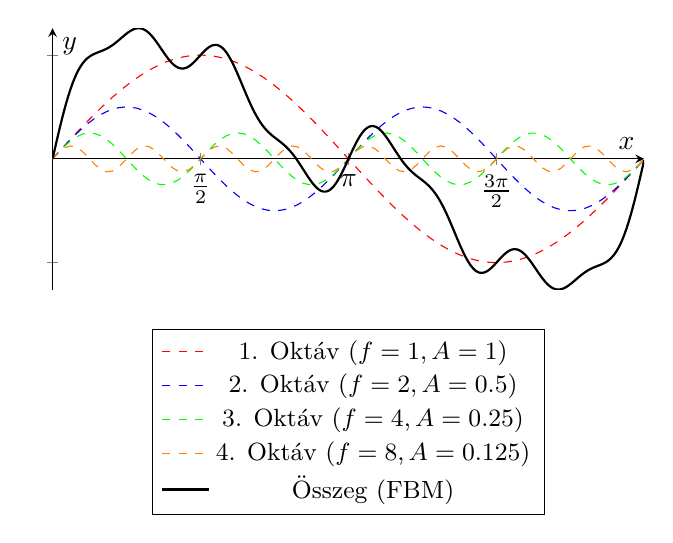
\begin{tikzpicture}[scale=1]
        \begin{axis}[
                width=0.75\textwidth,
                height=4.9cm,
                axis lines = middle,
                xlabel = $x$,
                ylabel = $y$,
                yticklabels={,,},
                xtick={1.5708, 3.14159, 4.71239, 6.28318},
                xticklabels={$\frac{\pi}{2}$, $\pi$, $\frac{3\pi}{2}$, $2\pi$},
                legend style={
                        at={(0.5,-0.15)}, anchor=north, font=\small } ]

            \addplot [domain=0:6.28, samples=100, color=red, dashed] {1.0 * sin(deg(x))};
            \addlegendentry{1. Oktáv ($f=1, A=1$)}

            \addplot [domain=0:6.28, samples=100, color=blue, dashed] {0.5 * sin(deg(x * 2))};
            \addlegendentry{2. Oktáv ($f=2, A=0.5$)}

            \addplot [domain=0:6.28, samples=100, color=green, dashed] {0.25 * sin(deg(x * 4))};
            \addlegendentry{3. Oktáv ($f=4, A=0.25$)}

            \addplot [domain=0:6.28, samples=100, color=orange, dashed] {0.125 * sin(deg(x * 8))};
            \addlegendentry{4. Oktáv ($f=8, A=0.125$)}

            \addplot [domain=0:6.28, samples=300, color=black, thick]
            {1.0 * sin(deg(x)) + 0.5 * sin(deg(x * 2)) + 0.25 * sin(deg(x * 4)) + 0.125 * sin(deg(x * 8))};
            \addlegendentry{Összeg (FBM)}
        \end{axis}
    \end{tikzpicture}
    \caption{Az oktávok összegzésének szemléltetése egy dimenzióban a szinuszfüggvénnyel.}
\end{figure}
\subsection{FBM pszeudókód}
A megvalósított kódban a fraktálzajt normalizáljuk a $[-1;1]$ intervallumra a
maximális lehetséges értékkel való osztással. A normalizálás után két saját
paramétert alkalmazunk.
\begin{itemize}[noitemsep]
    \item \textbf{Kontraszt:} A normalizált érték abszolútértékét erre a hatványra emeljük az eredeti előjel megtartásával. Így nagyobb lesz a kontraszt a nagyságok között.
    \item \textbf{Zajméret:} A kontraszt alkalmazása után ezzel az értékkel megszorozzuk a zaj értékét.
\end{itemize}
A fraktálzaj pszeudókódban megvalósítva:

\begin{algorithm}
    \linespread{1.0}\selectfont
    \caption{Fractal Brownian Motion (FBM)}
    \DontPrintSemicolon
    \Komment{A zaj paraméterei:}
    \Konstansok{oktavok, kontraszt: Egész}
    \Konstansok{frekvencia, amplitudo, persistence, lacunarity, zajMeret: Valós}
    \;
    \Fuggveny{FBM(\textbf{Konstans}: $x, y$: Valós) : Valós}{
        \Valtozok{zajErtek, maxErtek, jelenlegiAmplitudo, jelenlegiFrekvencia, zajElojel: Valós}
        \Valtozok{i: Egész}
        zajErtek $\coloneqq 0$\\
        maxErtek $\coloneqq 0$\\
        jelenlegiAmplitudo $\coloneqq$ amplitudo\\
        jelenlegiFrekvencia $\coloneqq$ frekvencia\\
        \;
        \Ciklus{$i \coloneqq 1$-től $oktavok$-ig}{
            \Komment{Zaj hozzáadása az aktuális frekvenciával és amplitúdóval}
            zajErtek $\coloneqq$ zajErtek + Zaj($x * jelenlegiFrekvencia$, $y * jelenlegiFrekvencia$) $*$ jelenlegiAmplitudo\\
            \;
            \Komment{Maximális lehetséges érték}
            maxErtek $\coloneqq$ maxErtek + jelenlegiAmplitudo\\
            \;
            \Komment{Paraméterek frissítése a következő oktávhoz}
            jelenlegiAmplitudo $\coloneqq$ jelenlegiAmplitudo $*$ persistence\\
            jelenlegiFrekvencia $\coloneqq$ jelenlegiFrekvencia $*$ lacunarity
        }
        \;
        \Komment{Normalizálás, kontraszt alkalmazása és méretezés}
        zajElojel $\coloneqq$ Elojel(zajErtek) \\
        \textit{FBM} $\coloneqq$ $(Abs(zajErtek / maxErtek))^{kontraszt} * zajElojel * zajMeret$
    }
\end{algorithm}
\newpage
\printbibliography[heading=bibintoc,title={Forrásjegyzék}]

\end{document}